%----------------------------------------------%
%                                              %
% Title:  Linux device drivers explained       %
% Author: Giuseppe Calderaro                   %
% Date:   29th October 2009                    %
%                                              %
%----------------------------------------------%

% Latex document class
\documentclass{beamer}
\usepackage{beamerthemeshadow}
\usepackage{listings}
\lstset{language=C}
\setbeamertemplate{navigation symbols}{}
\usetheme{Berkeley}
\beamersetuncovermixins{\opaqueness<1>{25}}{\opaqueness<2->{15}}

% Document start
\begin{document}
\title{Linux Device Drivers explained}
\author{Giuseppe Calderaro}
\institute[http://www.imgtec.com/]{Imagination technologies ltd.}
\date{29th October 2009}

% Slide: 1
\frame{\titlepage}

% Slide: 2
\frame{\frametitle{Table of contents}\tableofcontents}

%% LINUX SYSTEM ARCHITECTURE
% Slide: 3
\section{Linux system architecture}
\subsection{Linux system architecture}
\frame{\frametitle{Linux system architecture}
  \begin{columns}
    \begin{column}{10cm}
      \begin{figure}
        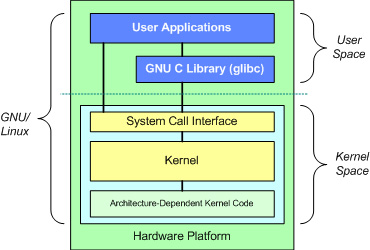
\includegraphics[scale=0.75]{arch1.eps}
        \caption{Linux system architecture}
      \end{figure}
    \end{column}
  \end{columns}
}

% Slide: 4
\subsection{Linux kernel architecture}
\frame{\frametitle{Linux kernel architecture}
  \begin{columns}
    \begin{column}{3cm}
      \begin{figure}
        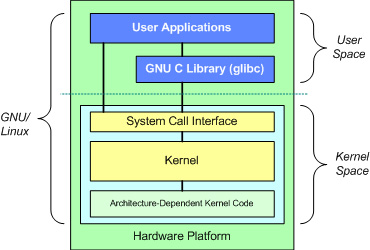
\includegraphics[scale=0.35]{arch1.eps}
        \caption{\tiny{Linux system architecture}}
      \end{figure}
    \end{column}
    \begin{column}{7cm}
      \begin{figure}
        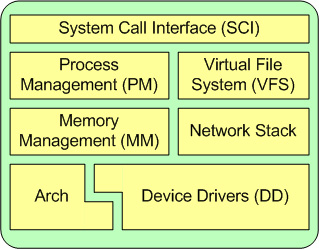
\includegraphics[scale=0.65]{arch2.eps}
        \caption{Linux kernel architecture}
      \end{figure}     
    \end{column}
  \end{columns}
}

%% BUILDING AND RUNNING MODULES
% Slide: 5
\section{Building and running modules}
\subsection{A polite module...}
\frame{\frametitle{A polite module...}
  \makebox{
    \scriptsize{
      \lstinputlisting{example.c}
    }
  }
}

% Slide: 6
\subsection{...and his Makefile}
\frame{\frametitle{...and his Makefile}
  \makebox{
    \scriptsize{
      \lstinputlisting{Module_Makefile}
    }
  }
}

%% DEBUGGING TECHNIQUES
% Slide: 7->9
\section{Debugging techniques}
\subsection{printk}
\frame{\frametitle{printk}
  \begin{itemize}
    \item<1-> printf(''I am printf!'');
    \item<2-> printk(''I am printk!'');
    \item<3-> printf prototype: int printf(const char *format, ...);
    \item<3-> printk prototype: int printk(const char *fmt, ...);
  \end{itemize}
}

% Slide: 10->11
\subsection{Log level values}
\frame{\frametitle{Log level values}
  \begin{itemize}
    \item<1-> \lstinputlisting{kernel_1line.h}
    \item<2-> \lstinputlisting{kernel_2line.h}
  \end{itemize}
}

% Slide: 12
\frame{\frametitle{Log level values}
  \makebox{
    \scriptsize{
      \lstinputlisting{kernel.h}
    }
  }
}

% Slide: 13->15
\subsection{mmm... proc... what's that?!?}
\frame{\frametitle{mmm... proc... what's that?!?}
  \begin{itemize}
  \item<1->{
    [giuseppe@wopr ~]\$ cat /proc/sys/kernel/printk\\
    3\hspace{1.5cm}4\hspace{1.5cm}1\hspace{1.5cm}7
  }
  \item<2-> Current Default Minimum Boottime
  \item<3-> echo 8 > /proc/sys/kernel/printk
  \item<3-> if the value is set to 8, all messages, including debugging ones, are displayed.
  \end{itemize}
}

% Slide: 16
\subsection{Other debugging techniques}
\frame{\frametitle{Other debugging techniques}
  \begin{itemize}
    \item Use the /proc filesystem
    \item Use ioctl method
    \item Debugging by watching (strace, ltrace)
    \item Oops messages (continues...)
    \item gdb vmlinux /proc/kcore
    \item kdb kernel debugger
    \item kgdb kernel debugger (in vanilla)
    \item User mode linux (!?!)
    \item Linux Trace Toolkit
    \item Kernel probes (good good)
    \item ice kernel debugger (waited for 4891AD)
  \end{itemize}
}

% Slide: 17
\subsection{OOOOOOOPS!}
\frame{\frametitle{OOOOOOOPS!}
  \tiny{
    \lstinputlisting{oops.txt}
  }
}

% Slide: 18
\section{Concurrency and Race conditions}
\subsection{Semaphores and mutexes}
\frame{\frametitle{Semaphores and mutexes}
  
}

% Slide: 19
\subsection{Reader/writer Semaphores}
\frame{\frametitle{Reader/writer semaphores}
  
}

% Slide: 20
\subsection{Completions}
\frame{\frametitle{Completions}
  
}

% Slide: 21
\subsection{Spinlocks and...}
\frame{\frametitle{Spinlocks and...}
  
}

% Slide: 22
\subsection{...Atomic Context!}
\frame{\frametitle{...Atomic Context!}
  
}

% Slide: 23
\subsection{Reader/Writer Spinlocks}
\frame{\frametitle{Reader/Writer Spinlocks}
  
}

% Slide: 24
\subsection{Locking Traps}
\frame{\frametitle{Locking Traps}
  
}

% Slide: 25
\subsection{Lock-Free Algorithms}
\frame{\frametitle{Lock-Free Algorithms}
  
}

% Slide: 26
\subsection{Atomic Variables}
\frame{\frametitle{Atomic Variables}
  
}

% Slide: 27
\subsection{Bit Operations}
\frame{\frametitle{Bit Operations}
  
}

% Slide: 28
\subsection{seqlocks}
\frame{\frametitle{seqlocks}
  
}

% Slide: 29
\subsection{Read-Copy-Update}
\frame{\frametitle{Read-Copy-Update}
  
}

% Slide: 30
\subsection{Title}
\frame{\frametitle{Title}
  
}

% Document end
\end{document}
